\chapter{Velocity and Angle estimation}
To give a better position estimate which can be fed to the controller as well, the different data collected from the sensors mounted are put through a \ac{KF}. This filter takes the different measurements as inputs, and uses these to give a better estimate of the position, rather than the quite noisy measurements taken using just the raw \ac{GPS} data. 

To develop such a filter, the model of the ship is to be computed, as well as a mapping of the different inputs and outputs to the system. The model of the forward and sidewards case (surge and sway) are the same as for the discrete system. 

\subsection{State model}
The state model is used as a base for computing the influence the different inputs have on the system. The matrix is the same as the $\vec{A}$ matrix used to describe the state space representation of the system. The general state expression is given as:
\begin{align}
\vec{x}(k) = \vec{\Phi}(k)\vec{x}(k-1) + \vec{w}(k)
\end{align}
\noindent Where:
\begin{ffk}
$\vec{\Phi}(k)$ is the state matrix\\
$\vec{x}(k-1)$ is the last input to the system\\
$\vec{w}(k)$ is the driving noise (the system input)
\end{ffk}
In this case, the driving noise $\vec{w}(n)$ will be the inputs to the system, which can then be used to estimate the different states. The states to be estimated is the velocity $\dot{x}$, the angular velocity $\omega$ and the angle of the vessel in the local frame $\theta$. The driving noise (or input) can be defined as the $\vec{B}$ matrix in the state system, multiplied with the different inputs given to the system, namely $n_1$ and $n_2$. When inserted, the formula for the state model becomes:
\begin{align}
\vec{x}(k) = \vec{\Phi}(k)\vec{x}(k-1) + \vec{B}\cdot\vec{u}
\end{align}

\subsection{Observation model}
The observation model, is a model that models the different observations. In this case, the different observations are measured directly, as we can measure both the angular velocity, the angle and the velocity of the craft. The general formula for the observation model is given as:
\begin{align}
\vec{z}(k) = \vec{H}(k)\vec{x}(k) + \vec{v}(k)
\end{align}
\noindent Where:
\begin{ffk}
$\vec{H}(n)$ is the model linking the measurements to the observations\\
$\vec{v}(n)$ is the measurement noise on the sensors
\end{ffk}
The noise from the measurements is estimated using previous measurements which can be used to estimate the variance and the mean of the measurements. The noise can in general be seen as zero-mean Gaussian white noise processes, which makes for the assumption:
\begin{align}
\vec{w}(n) \sim \mathcal{N}(0,\sigma_Z^2)
\end{align}
As $\vec{x}(n)$ is a row vector, $\vec{w}(n)$ is also a row vector with the same dimension. This calls for different variances on the different noise additions, for each of the measurements. As the variance of the noise on the \ac{IMU} is a lot bigger than on the \ac{GPS}. As all the measurements are available directly, the $\vec{H}(n)$ matrix is equal to identity. Giving the final observation model:
\begin{align}
\vec{z}(n) = \vec{x}(n) + \vec{v}(n)
\end{align}

% Wouldn't it be a fair assumption that a GPS doesn't have zero-mean, but has a wandering mean that would wander over time? 

% Text about the vector Kalman filer
% Text about the covariance matrix of such a system
\subsection{The Covariance matrices}
As the \ac{KF} is given as a vector \ac{KF}, the covariance matrices is to be computed. The definition for a covariance matrix is given as:
\begin{align}
Cov(\vec{X},\vec{X}) = \text{E}\langle[\vec{X} - \vec{\mu}_X][\vec{X} - \vec{\mu}_X]^\text{T}\rangle
\end{align}
The covariance matrix is used to tune the \ac{KF}, and weighs the different inputs according to the noise they experience. An assumption is to keep this constant. For the vector \ac{KF} there are two noises added to the system, one depicts the measurement noise, and the other the system noise. The system noise is in this project considered the input to the system. This can therefore be seen as the covariance of the input signals to the ship. As seen in \todo{insert reference to worksheet once its done -rlc} the distributions of the input signal $\vec{u}(k)$ can be seen as:
\begin{align}
F \sim \mathcal{N}(5.3544,55)\\
\tau \sim \mathcal{N}(0,20)
\end{align}
The covariance of these inputs, are then multiplied with $\vec{B}$ to give the input to the system $\vec{w}(k)$. As the two inputs are independent, the covariance matrix collapses to a matrix with diagonal entries, which gives the following matrix:
\begin{align}
Cov(\vec{X},\vec{X})_{3,3} = \sigma_{F}^2\\
Cov(\vec{X},\vec{X})_{9,9} = \sigma_{\tau}^2
\end{align}
When the system is simulated it gives the following response for estimating the position.
\begin{figure}[htbp]
	\centering
	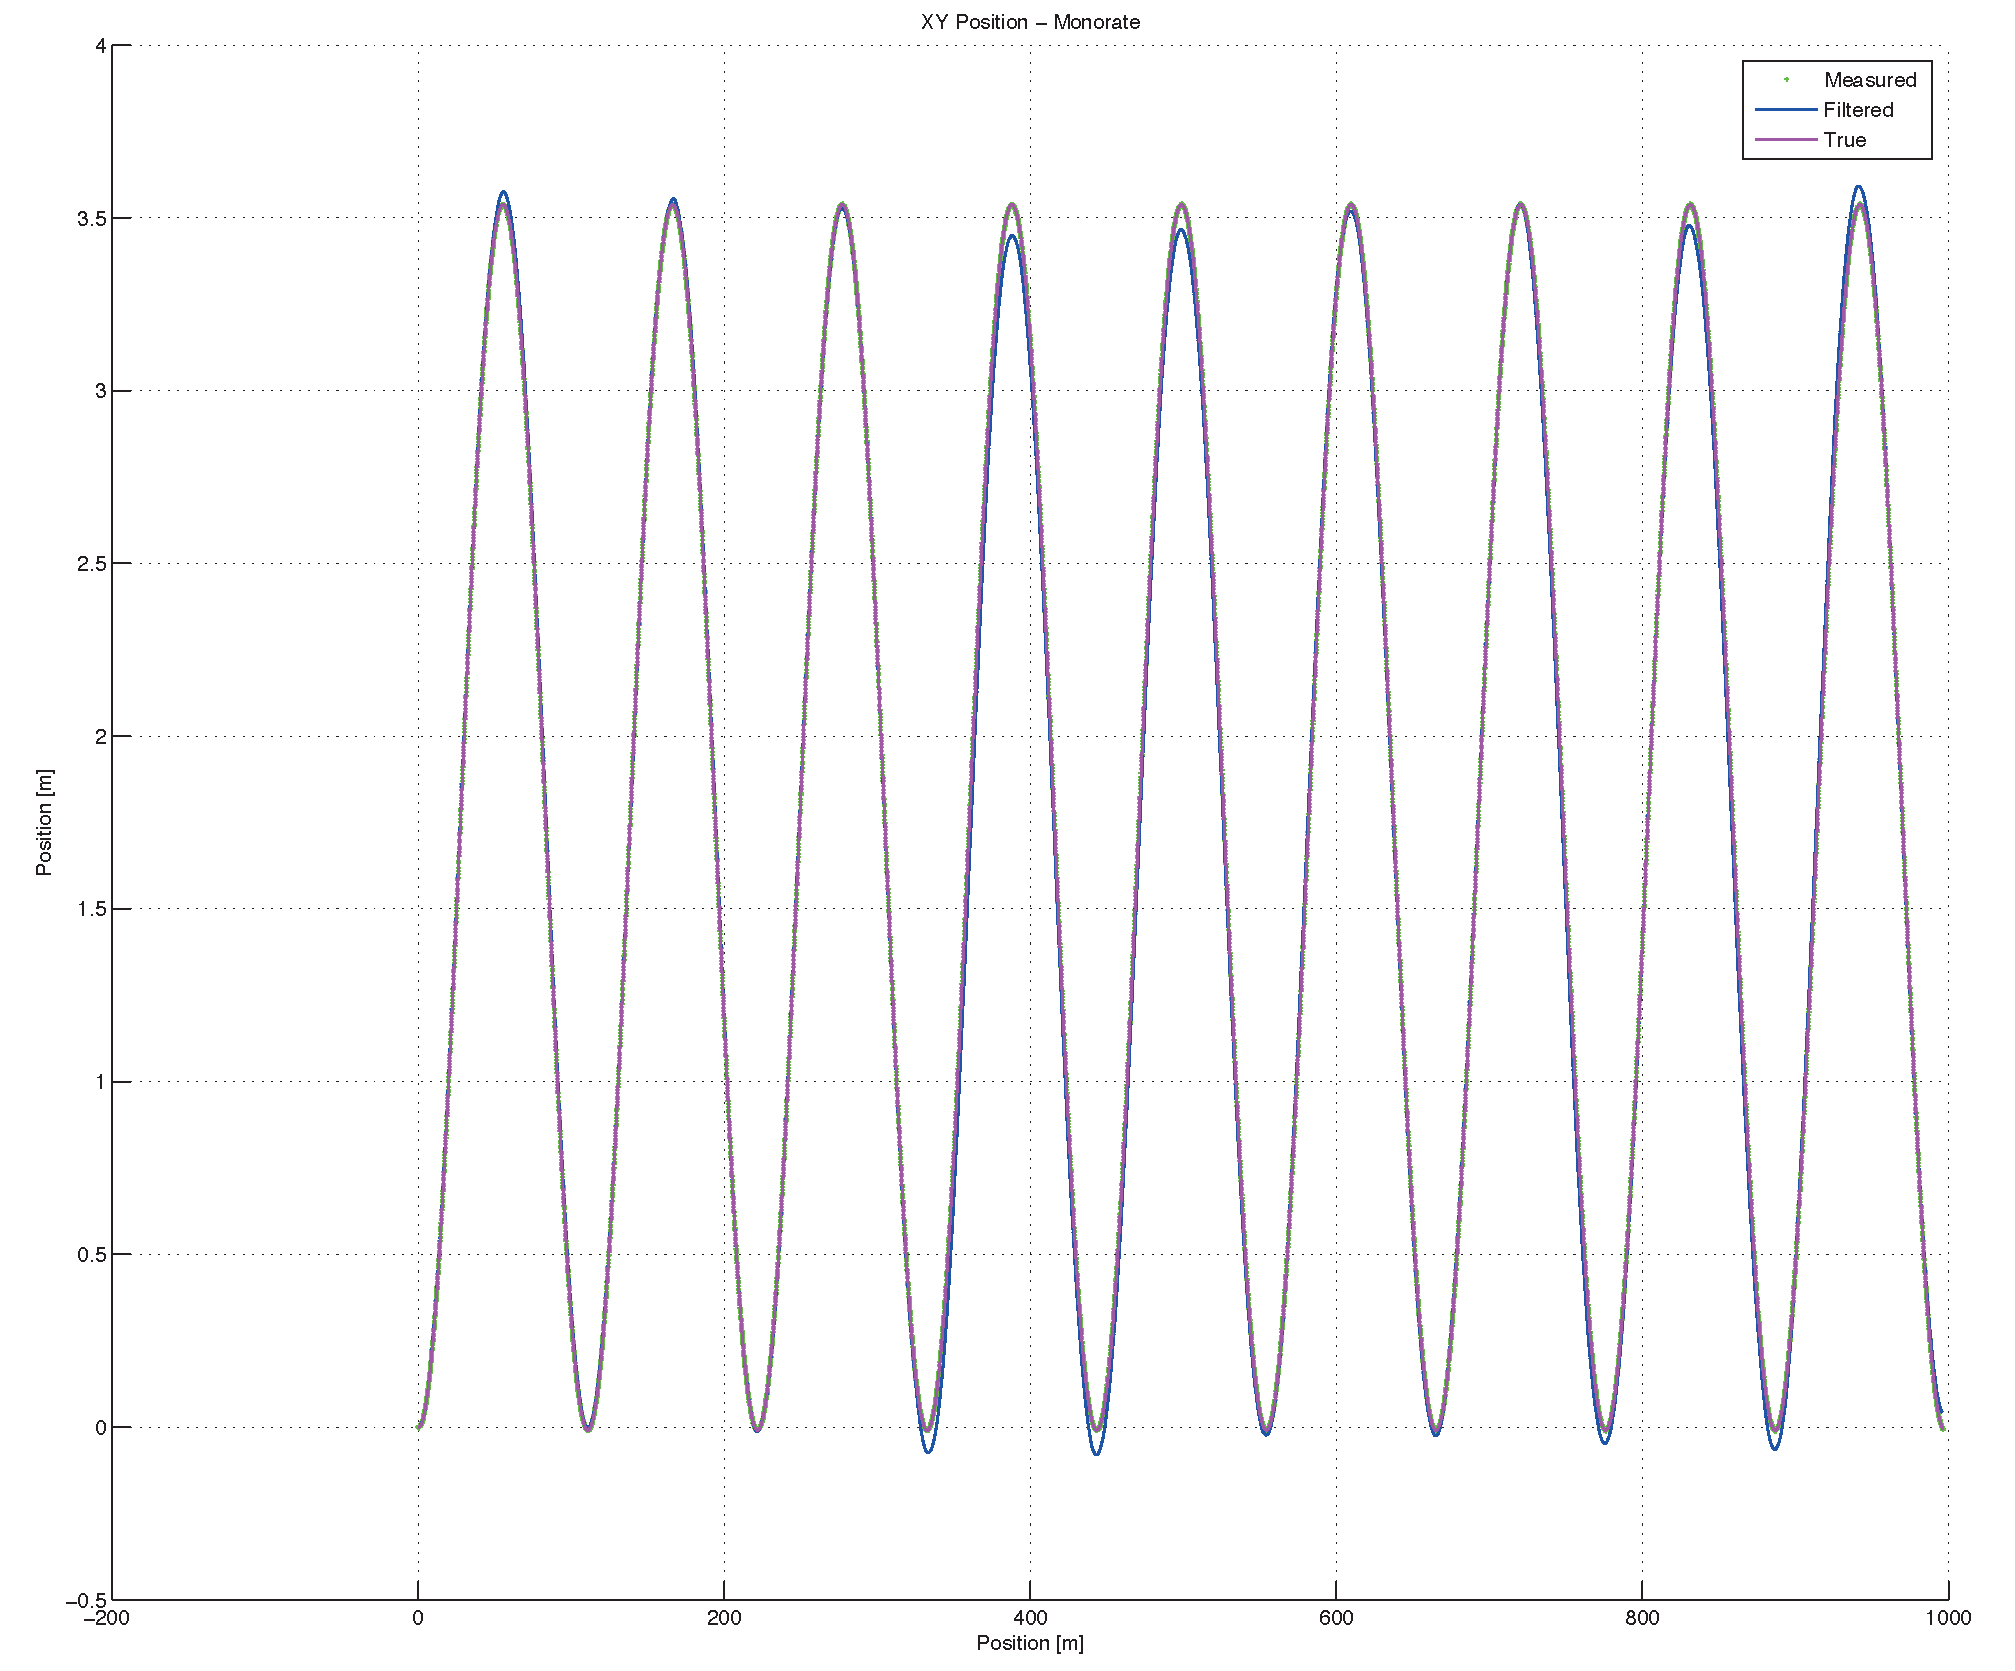
\includegraphics[width=\textwidth]{img/kalmana}
	\caption{Test to see if the \ac{KF} estimates the position}
	\label{fig:kalmanA}
\end{figure}
Figure\vref{fig:kalmanA} depicts how the system responds when running the measurements at the same sample rate. However - the \ac{GPS} only samples at 1Hz and the \ac{IMU} samples at 10Hz, the filter needs to be changed. The \ac{KF} must account for this change, which can be done by setting the noise of the measurement to a high value, which in turn will reduce the Kalman gain \todo{insert name of matrix -rlc} to zero, or just set the Kalman gain to zero. Both methods provide different results, as the estimate would then converge towards the last fixed value, whilst setting it to zero, would make the system use the other measurements available to the filter, and thus given an estimate, rather than convergin towards a fixed value. 	

\begin{align}
\vec{x}(n+1) = \vec{\Phi}\cdot\vec{x}(n) = \begin{bmatrix}
1 & t_s & \frac{t_s^2}{2} & 0 & 0 & 0 & 0 & 0 & 0\\
0 & 1 & t_s & 0 & 0 & 0 & 0 & 0 & 0\\
0 & -\beta_X & 0 & 0 & 0 & 0 & 0 & 0 & 0\\
0 & 0 & 0 & 1 & t_s & \frac{t_s^2}{2} & 0 & 0 & 0\\
0 & 0 & 0 & 0 & 1 & t_s & 0 & 0 & 0\\
0 & 0 & 0 & 0 & -\beta_Y & 0 & 0 & 0 & 0\\
0 & 0 & 0 & 0 & 0 & 0 & 1 & t_s & \frac{t_s^2}{2}\\
0 & 0 & 0 & 0 & 0 & 0 & 0 & 1 & t_s\\
0 & 0 & 0 & 0 & 0 & 0 & 0 & -\beta_\omega & 0\\
\end{bmatrix}\begin{bmatrix}
x(n)\\
\dot{x(n)}\\
\ddot{x(n)}\\
y(n)\\
\dot{y(n)}\\
\ddot{y(n)}\\
\theta(n)\\
\omega(n)\\
\alpha(n)\\
\end{bmatrix}
\label{eq:matr}
\end{align}
In \vref{eq:matr} the system matrix is seen to be 3 individual systems. The inputs to the \ac{KF} is the desired force (computed by the controller) and the measurements given by the sensors mounted about the ship. The desired inputs to the system are put through the $\vec{B}$ matrix, which converts these to an acceleration and an angular acceleration respectively. These are then used as a basis for computing the estimating the output of the system. 

\begin{align}
\vec{Z} = \begin{bmatrix}
0 & 0\\
0 & 0\\
\frac{1}{m} & 0\\
0 & 0\\
0 & 0\\
0 & 0\\
0 & 0\\
0 & 0\\
0 & \frac{1}{I}\\
\end{bmatrix}\begin{bmatrix}
F\\
\tau
\end{bmatrix}
\end{align}



On \vref{fig:revol} a test input to the system is plotted. The sequence is an alternating angle reference sequence, the angle is a sine curve. 
\begin{figure}[htbp]
	\centering
%	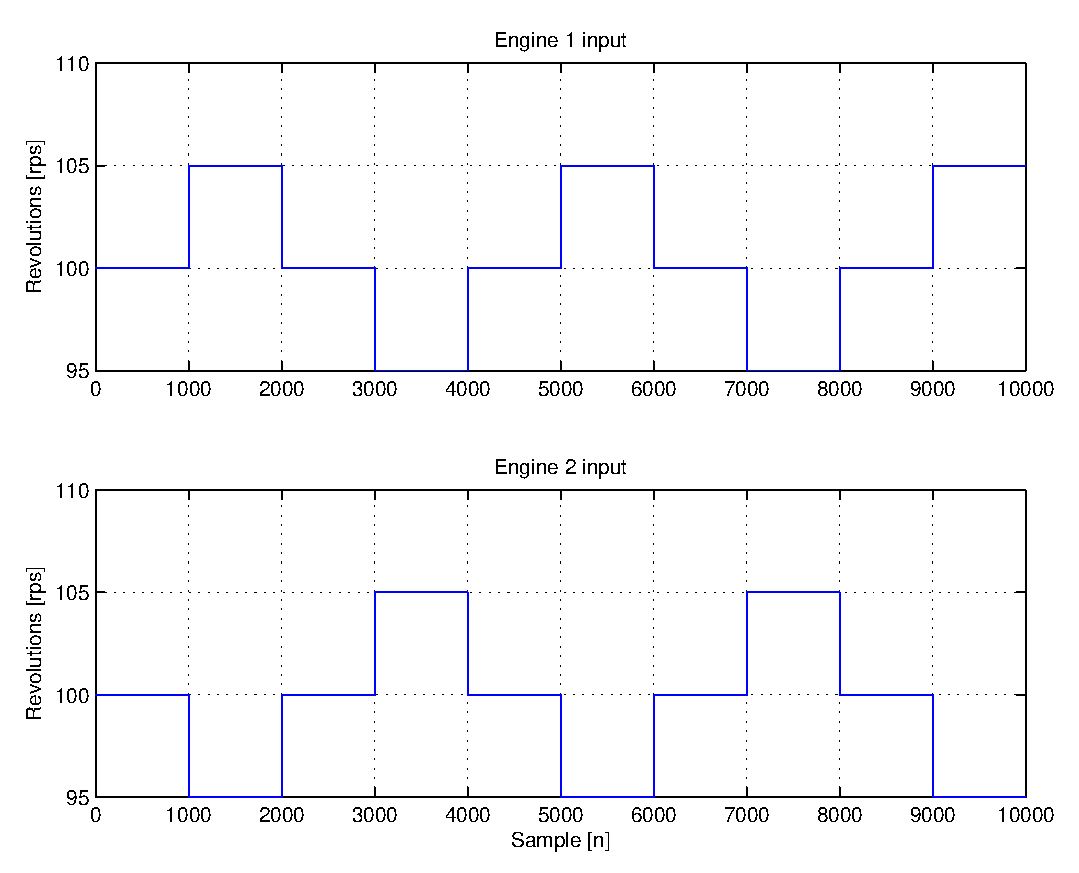
\includegraphics[width=\textwidth]{img/revol}
	\caption{Test input to the system}
	\label{fig:revol}
\end{figure}

As these cannot be measured accurately, we need to add noise to the input signals.

As the GPS have a different sampling rate than the \ac{IMU} the measurements are to be kept at zero if the 

Foreslag til Paper: Hvor langt ned kan man gå i sampling på GPS'en for at spare båndbredde, uden at miste præcision!

\subsection{Simulations of the filter}
Simulation of the \ac{KF} have proven to provide an accurate estimate, however - the actual variances have to be measured. 

To avoid computational problems the Joseph Form of the \ac{KF} can be used. This ensures that the matrices used in the updating step is non-singular and positive definite. 

If the filter is simulated, the following results are produced. 
\todo{insert filter pictures once we decided on final filter! -rlc}



\section{Position estimation}
During the development of the \ac{KF} a lot or problems were discovered. One is to estimate the variances of the different measurement devies. The GPS delivers a position in latitude longitude format - which is converted into an x and y coordinate by rotating the entire system and shifting the local frame of the ship as a surface tangent to the earth. This will of course only be an estimate, but as the curvature of the earth is relatively small. The distance to the horizon can be estimated by $d \approx 3.57\sqrt{h}$ which on the ground, equals that the distance to the horizon is approximately 3.57 kilometers. As the areas to be measured are defined by a local bounding box - this area will to be defined to be smaller than 3.5 kilometers.

This section will contain the different things we've considered during the miniproject in \ac{KF}ing, and will be used to give a better estimate of the actual position (from the measurements implemented on the ship).

Below is a description of the measurable inputs to the system. These are obtained from a \ac{GPS} and a \ac{IMU} mounted on the ship.
Position and velocity from the \ac{GPS}: rotated coordinates (from LatLon to Local frame)
Linear acceleration from the \ac{IMU}: accelerometer
Angular acceleration from the \ac{IMU}: gyrometer
Angle from the \ac{IMU}: magnetometer (compass)

\section{Estimation of position on a lossy channel}
As the controls are run on a remote platform, the \ac{KF} should be able to work even though some sensor measurements are corrupted. To work around this, the Kalman gain should be set to zero of the readout is corrupted - so every time the receiver gets a packet where the checksom is invalid, it generates a vector mask that tells which rows of the Kalman gain should be zeroed. 

To test this, \MATLAB has been used, which generates the the following results for a given packet loss rate. This rate can be then be altered to see how the system responds to a given data loss rate. The data loss rate is given in percent. If the system looses 10\% of the packages, the following error curves are produced:

The 4 figures represent the error with a 10 percent loss, a 20 percent loss, a 30 percent loss and finally a 40 percent loss in data. 